%% 
%% Copyright 2007, 2008, 2009 Elsevier Ltd
%% 
%% This file is part of the 'Elsarticle Bundle'.
%% ---------------------------------------------
%% 
%% It may be distributed under the conditions of the LaTeX Project Public
%% License, either version 1.2 of this license or (at your option) any
%% later version.  The latest version of this license is in
%%    http://www.latex-project.org/lppl.txt
%% and version 1.2 or later is part of all distributions of LaTeX
%% version 1999/12/01 or later.
%% 
%% The list of all files belonging to the 'Elsarticle Bundle' is
%% given in the file `manifest.txt'.
%% 
%% Template article for Elsevier's document class `elsarticle'
%% with harvard style bibliographic references
%% SP 2008/03/01

%% Use the option review to obtain double line spacing
\documentclass[preprint,review,11pt,authoryear]{elsarticle}
\usepackage{natbib}
\usepackage[hyphens]{url}
% To achieve 1.5 line spacing
\linespread{1.3}

%% Use the options 1p,twocolumn; 3p; 3p,twocolumn; 5p; or 5p,twocolumn
%% for a journal layout:
%% \documentclass[final,1p,times,authoryear]{elsarticle}
% \documentclass[final,1p,times,twocolumn,authoryear]{elsarticle}
%% \documentclass[final,3p,times,authoryear]{elsarticle}
%% \documentclass[final,3p,times,twocolumn,authoryear]{elsarticle}
%% \documentclass[final,5p,times,authoryear]{elsarticle}
%% \documentclass[final,5p,times,twocolumn,authoryear]{elsarticle}

%% For including figures, graphicx.sty has been loaded in
%% elsarticle.cls. If you prefer to use the old commands
%% please give \usepackage{epsfig}

%% The amssymb package provides various useful mathematical symbols
\usepackage{amsmath,amssymb}
% \usepackage[boxed,linesnumbered,ruled,algo2e]{algorithm2e}   % for algorithm box
\usepackage{algorithm}
\usepackage{algpseudocode}
%% The amsthm package provides extended theorem environments
\usepackage{amsthm}
%% For indicator function 1
\usepackage{bm, bbm, mathrsfs}
\usepackage{sansmath}
%\usepackage{todonotes}
%\usepackage[final,inline]{showlabels}
\usepackage{jm,ks}
\usepackage{float} % Required for using the H specifier
\usepackage{enumitem}
\usepackage{multicol}

\usepackage{longtable}
\usepackage{booktabs}
\makeatletter
\def\ps@pprintTitle{
  \let\@oddhead\@empty
  \let\@evenhead\@empty
  \let\@oddfoot\@empty
  \let\@evenfoot\@oddfoot
}
\makeatother

\begin{document}


\begin{frontmatter}

\title{Drone Delivery System in Post-Disaster Humanitarian Logistics: A Two-Stage Stochastic Programming Approach with Uncertain Wind Conditions}


\author[mymainaddress1]{Yuyang Ma}
\cortext[cor1]{Corresponding author. }
 \ead{yuyang.ma@lehigh.edu}
\address[mymainaddress1]{Department of Industrial and Systems Engineering, Lehigh University, Bethlehem, PA,  USA}



\begin{abstract}
\noindent This study extends the drone-based delivery system model proposed by \cite{dukkanci2023drones} by incorporating the effects of uncertain weather conditions, specifically wind, on the delivery process. We formulate the problem as a two-stage stochastic programming (SP) model and introduce a scenario decomposition algorithm (SDA) along with a cluster-based heuristic algorithm to address it. By including weather uncertainties, we achieve a more realistic assessment of drone delivery capabilities in post-disaster scenarios. Our computational experiments demonstrate that considering wind uncertainty significantly enhances the reliability and effectiveness of drone delivery systems in humanitarian logistics. Additionally, we consider the issue of fairness in the distribution of relief items by integrating equity constraints and objectives, ensuring a more balanced allocation of resources among affected populations. 

\begin{keyword} 
stochastic programming \sep drone delivery \sep uncertain wind condition \sep scenario decomposition algorithm 
\end{keyword}

\end{abstract}
\end{frontmatter}

\section{Introduction} \label{sec:introduction}
As drone technology has been rapidly developed, their application in various fields has been extensively studied. In the commercial delivery sector, leading organizations like \cite{ups2017drone} and \cite{amazon2022drone} have utilized drones to deliver packages. Additionally, drones have demonstrated their potential in humanitarian and healthcare operations. For example, in collaboration with other organizations, DHL successfully tested the delivery of medicines using a drone to an island in Lake Victoria. Due to poor infrastructure and difficult terrain, medical supplies for the approximately 400,000 residents of Ukerewe Island in Lake Victoria were severely limited. However, thanks to the advantages of drones, such as ignoring road conditions and rapid flying speed, the delivery time was successfully reduced from six hours to 40 minutes. Emergency deliveries in such areas are no longer an impossible mission (\cite{dhl2018drone}). Drones are also particularly suitable for mountain search and rescue operations (\cite{karaca2018potential}). Zipline, a famous delivery company, has been using drones to deliver medical supplies, including COVID-19 vaccines, to remote areas in Rwanda and Ghana. This innovative approach started in Ghana in early 2021, making it the first country to launch a nationwide program to deliver coronavirus vaccines using drones. The drones have also been used to transport personal protective equipment (PPE) and COVID-19 test samples from rural areas to labs in urban centers (\cite{Zipline2020}).

Even though drones can provide a comprehensive delivery network, there are still some challenges to be addressed. Compared to trucks, drones have significantly smaller payload and range limit. A diesel cargo van RAM Pro Master 2500 has 378 times the carrying capacity and nearly 20 times the range of a typical drone (\cite{figliozzi2017lifecycle}). Due to its limited range, a drone-based delivery system requires more depots or launching sites distributed across the region. Also, unexpected and/or adverse weather conditions, e.g., headwinds, may dramatically alter the energy consumption and/or range of a delivery drone. Besides, the range limit of drones decreases as the payload increases. 

Motivated by the applications mentioned before, in this study, we extend the post-disaster humanitarian application proposed by \cite{dukkanci2023drones}. In their study, a drone-based system is proposed to deliver medical supplies to earthquake-affected areas. After the earthquake, owing to the debris and potential collapse of roads, traditional transportation methods like trucks are not ideal for delivery. The system uses two types of drones to deliver the required emergency goods. Additionally, all deliveries must be completed within a certain time window. The objective is to minimize the total unmet demand. The authors formulated the problem as a mixed-integer linear programming (MILP) model and proposed a scenario decomposition algorithm (SDA) to solve it. However, their model included some unrealistic assumptions. For example, they neglected the effects of payload on the range limits of large drones. We use a formula to calculate the range of drones, which considers the payload, battery capacity, speed of drones, etc. They also assumed that weather conditions do not affect the process of drone delivery, which significantly deviates from real conditions. In this study, we consider uncertain weather conditions and their effects on the speed of drones.

Summarizing, our main contributions are the followings:
\vspace{-7pt}
\begin{enumerate}[label=$\bullet$, itemsep=0em]
    \item We consider the effects of uncertain wind conditions on the delivery process of drones.
    \item Introducing the cost of using drones, we add size of drone fleets in the decision process.
    \item We reformulate the problem as a two-stage stochastic programming problem and construct a scenario decomposition algorithm to solve it. We also propose a cluster-based heuristic algorithm to solve the problem. % Besides, the reason of poor performance of the Benders decomposition algorithm is discussed.
    \item Computational experiments are conducted to evaluate the performance of the proposed algorithm. An out-of-sample test is also conducted to verify the value of considering uncertain wind conditions. Additionally, 3 variations of the problem where the fairness issue is considered are discussed.
\end{enumerate}
\vspace{-7pt}

The remainder of this paper is organized as follows. In Section \ref*{sec:Review}, we review the literature related to our study. Next the settings of our problem and the new formulation we used are shown in Section \ref*{sec:formulation}. We describe different solution strategies in Section \ref*{sec:methods}. Section \ref*{sec:results} describes the process of generating uncertain demand, road distance based on the earthquake scenario, and presents a computational analysis. Finally, we conclude the paper in Section \ref*{sec:conclusion}

\section{Literature Review}\label{sec:Review}
In this section, we primarily focus on the literature related to facility location problems with drone delivery. For the comprehensive survey of drone delivery, we refer readers to \cite{dukkanci2023facility}. Unmanned autonomous vehicles (UAV), commonly referred to as drones, shows great potential in the field of logistics and transportation. The use of drones in logistics and transportation can significantly reduce the cost and time of delivery, compared to traditional delivery methods. The drone delivery problem is a new research area that has attracted increasing attention from researchers. \cite{murray2015flying} proposed two kinds of routing problem, where trucks and drones were used to achieve the last-mile delivery. The first was known as the flying sidekick traveling salesman problem (FSTSP), in which when a truck reached a customer, a drone launched from the truck to serve another customer and subsequently returned to the truck at the depot or another customer location. The second problem proposed is known as the parallel drone-scheduling traveling salesman problem. In this case, a truck and drones operated separately, such that the truck was routed between customers and the drones performed dedicated deliveries. Both problems aimed to minimize the latest arrival time of the truck or drone at the depot. \cite{murray2020multiple} extended the FSTSP, where multiple drones launched form the truck to serve customers and the objective is to minimize the last return time of the truck or drone to the depot. 

Besides the FSTSP mentioned before, a substantial amount of literature exists on maximal covering facility location problem (MCFLP) (\cite{church1974maximal}), where the decision maker needs to decide where the facilities open so that the demand of customers covered by the delivery network is maximized. Both \cite{farahani2012covering} and \cite{owen1998strategic} provided comprehensive review on this kind of problem and corresponding solution strategies. \cite{chauhan2019maximum} extended MCFLP as using drones to be the only delivery method. In their model, they considered the payload and range limit of drones, and they explicitly calculated the energy consumption of drones as a function of the distance of delivery and payload. The objective was to maximize the covering weighted demand. They formulated the problem as a pure integer programming model and proposed a heuristic algorithm to solve it. \cite{zhu2022two} focused on a short-term post-disaster humanitarian relief application using unmanned aerial vehicles (UAVs) to deliver first-aid products to customer demand points. The problem was framed as a two-stage robust facility location problem with drones (two-stage RFLPD), incorporating demand uncertainty through various demand scenarios. The objective was to develop a location-allocation-assignment plan that minimized the two-stage total cost in the worst-case scenario of all possible demand outcomes. They proposed three different models of this problem, two of which integrated a realistic UAV electricity consumption model, while the third offered greater operational flexibility. The column-and-constraint generation method and Benders decomposition were employed to solve the models. In \cite{dukkanci2023drones}, authors proposed a two-echelon delivery system where drones were used to achieve the last-mile delivery and trucks were used to store packages and carry small drones. The goal they aimed to achieve, minimizing the total unmet demand, has a similar spirit to maximizing the covering weight demand. However, the problem in \cite{dukkanci2023drones} was more complicated than the aforementioned MCFLP, as they considered the uncertainty of demand and road networks. Besides, they also included the time-window constraint into the model. As for the solution strategy, they proposed a scenario decomposition algorithm to solve the problem. 

In this study, we further extend the model proposed by \cite{dukkanci2023drones} by considering the effects of uncertain wind conditions on the delivery process of drones. Besides, \cite{dukkanci2023drones} assumed a pre-specified number of drones were assigned to each open facility, whereas in our model, we consider the size of drone fleets as decision variables. The additional drone usage feature adds to the complexity of the formulation. Our problem also function aimed at minimizing the unsatisfied demand and cost induced by usage of drones under uncertainty within a predetermined time bound, which has not been considered in any other related studies in the literature.

\section{Problem Description and Mathematical Formulations}\label{sec:formulation}
\subsection{Problem Statement} \label{subsec:ProblemStatement}
After the earthquake, the road connections between the supply points and gathering points, where the affected people gathers, may be disrupted. In this situation, drones can serve as the primary delivery method for distributing relief items to affected people. We use the same two-echelon delivery system proposed by \cite{dukkanci2023drones}. This system includes two types of drones—small drones and large drones—and trucks. Both types of drones have limited payload capacities and delivery ranges. There are two types of locations related to the drones: depots and launch points. Depots store the drones and relief items, while launch points are used to park the trucks. Due to more comprehensive function and scale, we assume that we will open more launch points than depots. Trucks can also store a certain amount of relief items and serve as launch platforms for small drones. At the first echelon, trucks carry relief items and small drones from depots to launch points, and small drones will finish the last-mile delivery. In contrast, at the second echelon, both small drones and large drones deliver the relief items to gathering points directly from depots. A sample of the proposed drone delivery system is shown in Figure \ref{fig:drone_delivery_system}.

\begin{figure}[h!]
    \centering
    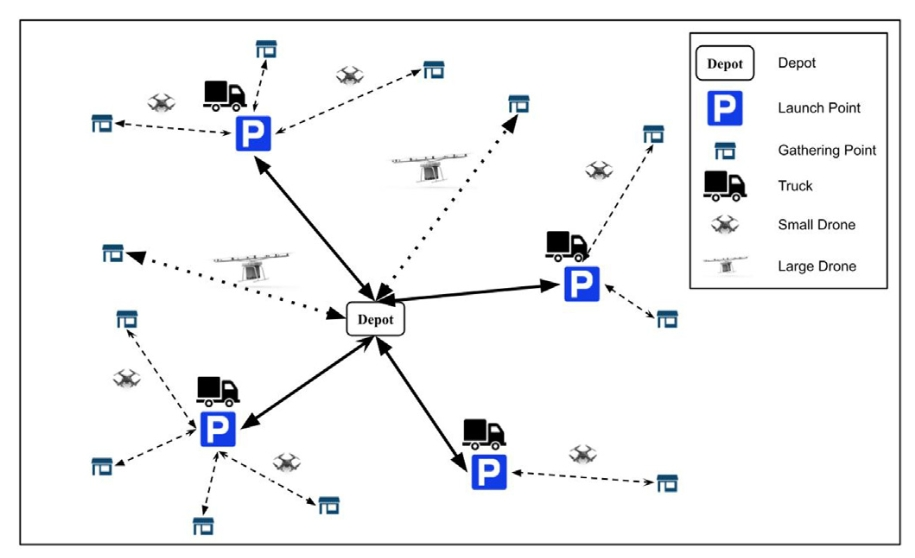
\includegraphics[width=0.7\linewidth]{Drone_delivery_system.png}
    \caption{Proposed drone delivery system by \cite{dukkanci2023drones}}
    \label{fig:drone_delivery_system}
\end{figure}

One of the main reasons for the devastating impact of earthquakes is their unpredictability. Specifically, the time, place, and magnitude of earthquakes cannot be predicted. Consequently, the number of relief items required by affected people and the impact on the road network are uncertain before an earthquake occurs. Therefore, we consider the uncertainties of demand and road networks. Except for the aforementioned range and payload limit of drones, a time-window constraint is also introduced to ensure that all the deliveries are completed within a certain time frame due to the emergency. To ensure that relief items are delivered to the maximum number of people, minimize the total unsatisfied demand at all gathering points is a critical part of the objective. Moreover, the cost induced by using drones should also be seriously considered. Therefore, our objective function consists of two parts: the penalty of unsatisfied demand and the cost of using drones. The problem can be formulated as a two-stage stochastic programming model. In the first stage, the decision maker needs to determine which the depots and launch points are to open, and the assignment of launch points to depots. After the earthquake happens, the damage to the road connections and demand of each gathering points will reveal. In the second stage, the decision maker needs to decide the number of each type of drone to use, the assignment of drones to gathering points, and coherently unmet demand at each gathering point can be calculated.

\subsection{Mathematical Formulation} \label{subsec:MathematicalFormulation}
We consider this problem as a two-stage stochastic programming problem. In the first-stage, the decision maker is given a set of potential gathering points $I$, a set of locations for potential depots $D$, a set of locations for potential launch points $L$, and two sets of available drones $K_{SD}$ for the small drones, and $K_{LD}$ for large drones. The first-stage decision variables are $u_d$, $v_l$, and $w_{ld}$, which represent the decision of opening a depot at location $d$, opening a launch point at location $l$, and assigning launch point $l$ to depot $d$, respectively. The second-stage decision variables are $g_k$, $x_{ilk}$, $y_{idk}$, and $o_i$, which represent the decision of using drone $k$, assigning small drone $k$ to serve point $i$ from location $l$, assigning large drone $k$ to serve point $i$ from depot $d$, and the unmet demand for gathering point $i$, respectively. The objective function of the first-stage problem is to minimize the expected cost of the second-stage problem. The first-stage problem is subject to constraints on the number of open depots and launch points, and the assignment of launch points to depots. The second-stage problem is to minimize the expected cost of using drones, the penalty for unmet demand, and the cost of using drones. The second-stage problem is subject to constraints on the assignment of drones to gathering points, the capacity of trucks, the capacity of small drones, the capacity of large drones, the unmet demand, and the assignment of launch points to depots. The mathematical notation used in the formulation is given in Table \ref{table:notation}. 
\begin{table}[h!]  
\center
\renewcommand{\arraystretch}{1.2}
\caption{Notation}\resizebox{\textwidth}{!}{ % <--- resizebox function requires package: graphicx
\begin{tabular}{ll}
\toprule 
\multicolumn{2}{l}{\textbf{Sets}} \\
$I$                           & Set of gathering points                                                                    \\
$D$                           & Set of potential depot locations                                                           \\
$L$                           & Set of potential depot locations                                                           \\
$K_{SD}$                      & Set of available small drones                                                              \\
$K_{LD}$                      & Set of available Large drones                                                              \\
\multicolumn{2}{l}{\textbf{Parameters}} \\
$e$                           & Maximal number for open depots                                                             \\
$p$                           & Maximal number for open launch points                                                      \\
$Q_T$                         & Capacity of Trucks                                                                         \\
$Q_{SD}$                      & Capacity of small drones                                                                   \\
$Q_{LD}$                      & Capacity of large drones                                                                   \\
$c_{SD}$                      & Cost of using small drones                                                                 \\
$c_{LD}$                      & Cost of using large drones                                                                 \\
$v_T$                         & Speed of trucks                                                                            \\
$v^{SD}$                      & Speed of small drones                                                                      \\
$v^{LD}$                      & Speed of large drones                                                                      \\
$v^{w}$                       & Speed of wind                                                                              \\
$\alpha^{w}$                  & Direction of wind                                                                          \\
$T$                           & Length of time period                                                                      \\
$\tau$                        & Preparation time for small drones                                                          \\
$\omega_{ld}$                 & Ground distance between depot $d$ and launch point $l$ after the earthquake                \\
$q_i$                         & Demand at gathering point $i$                                                              \\
$\pi$                         & Penalty per unit of unmet demand                                                           \\
\multicolumn{2}{l}{\textbf{First-stage decision variables}}                                                                \\
$u_d$                         & 1, if a depot is open at location $d \in D$, 0 otherwise                                   \\
$v_l$                         & 1, if a launch point is open at location $l \in L$,0 otherwise                             \\
$w_{ld}$                      & 1, if launch point $l$ is assigned to depot $d$, 0 otherwise                               \\
\multicolumn{2}{l}{\textbf{Second-stage decision variables}}                                                               \\
$g_k$                         & 1, if a drone $k \in \{K_{SD} \cup K_{LD}\}$ is used, 0 otherwise                          \\
$x_{ilk}$                     & 1, if a small drone $k \in K_{SD}$ is assigned to serve point $i \in I$ from location $l \in \{L \cup D\}$, 0 otherwise \\
$y_{idk}$                     & 1, if a large drone $k \in K_{LD}$ is assigned to serve point $i \in I$ from depot $d \in D$, 0 otherwise \\
$o_i$                         & Unmet demand for gathering point $i \in I$                                                 \\
\bottomrule
\end{tabular}
}
\label{table:notation}
\end{table} 
Our stochastic programming formulation consists of two stages. In the first stage, the decision-maker determines the locations of depots and launch points, and assign launch points to depots. After this stage, the earthquake occurs, revealing the true values of demands, weather information and the damage percentage of the road network. In the second stage, the agent must decide the number of drones to use, assign drones to gathering points, and determine the unmet demand at each gathering point. The first-stage problem is formulated as follows:
\footnotesize
\begin{subequations} \label{formulation:1stStage}
    \begin{align}
        \min \quad & \E_{\P} \left[ Q(u,v,w,\xi) \right] && \label{objective:1stStageObj} \\
        \subjectto \quad & \sum_{d \in D} u_d \leq e     && \label{constraint:Num_Depot} \\
                         & \sum_{l \in L} v_l \leq p     && \label{constraint:Num_Launch} \\
                         & \sum_{d \in D} w_{ld} = v_l,  && \forall l \in L \label{constraint:LaunchPointtoOneDepot} \\
                         & w_{ld} \in \{0,1\}, && \forall d \in D, l \in L \label{constraint:wBinary} \\
                         & u_d \in \{0,1\}, && \forall d \in D \label{constraint:uBinary} \\
                         & v_l \in \{0,1\}, && \forall l \in L \label{constraint:vBinary}
    \end{align}
\end{subequations}
\normalsize
where the objective function (\ref{objective:1stStageObj}) is set to be minimizing the expectation the second stage's cost. The constraint (\ref{constraint:Num_Depot}) and (\ref{constraint:Num_Launch}) limit the number of depots and launch points that can be opened. The constraint (\ref{constraint:LaunchPointtoOneDepot}) ensures that each launch point is assigned to exactly at most one depot. The uncertainties in the second-stage decision are indicated as the parameter $\xi \in \Xi$, where $\xi = \left( \omega, q , v^{wind} , \alpha^{wind} \right)$. In stochastic programming, we assume that the random variable $\Xi$ is under a known distribution $\P$. The second stage problem is constructed as:
\footnotesize
\allowdisplaybreaks
\begin{subequations} \label{formulation:2ndStage}
    \begin{align}
        Q[u,v,w] :=  \quad \min \quad & \sum_{i \in I} \pi o_i + \sum_{k \in K_{SD}} c_{SD} g_k + \sum_{k \in K_{LD}} c_{LD} g_k & & \label{objective:2ndStageObj} \\
                     \subjectto \quad & y_{idk} \leq u_d && \forall d \in D, i \in I, k \in K_{LD} \label{constraint:DepotOpen1}\\
                                      & x_{ilk} \leq u_l && \forall l \in D, i \in I, k \in K_{SD} \label{constraint:DepotOpen2}\\
                                      & x_{ilk} \leq v_l && \forall l \in L, i \in I, k \in K_{SD} \label{constraint:LaunchPointOpen} \\
                                      & \sum_{i \in I} \sum_{l \in \{L \cup D\}}x_{ilk} \leq g_k && \forall k \in K_{SD} \label{constraint:SmallDrone_Usage}\\
                                      & \sum_{i \in I} \sum_{d \in D}y_{idk} \leq g_k && \forall k \in K_{LD} \label{constraint:LargeDrone_Usage}\\
                                      & \sum_{k \in K_{SD}} \sum_{i \in I} q_i x_{ilk} \leq Q_T v_l && \forall l \in L \label{constraint:TrucksCapacity} \\
                                      & q_i - \sum_{k \in K_{SD}}\sum_{l \in \{L \cup D\}} Q_{SD} x_{ilk} - \sum_{k \in K_{LD}}\sum_{d \in D} Q_{LD} y_{idk} \leq o_i && \forall i \in I \label{constraint:UnmetDemand} \\
                                      & \sum_{d \in D} \frac{\omega_{ld}}{v_T} w_{ld} + \sum_{i \in I} \left( \frac{2d_{li}}{v_{li}} + \tau \right) x_{ilk} \leq T && \forall l \in L, k \in K_{SD} \label{constraint:LPTimeLimitSD} \\
                                      & \sum_{i \in I} \left( \frac{2d_{li}}{v_{li}} + \tau \right) x_{ilk} \leq T && \forall l \in D, k \in K_{SD} \label{constraint:DepotTimeLimitSD} \\
                                      & \frac{2d_{ji}}{v_{ji}} y_{ijk} \leq T && \forall j \in D, i \in I, k \in K_{LD} \label{constraint:DepotTimeLimitLD} \\
                                      & g_k \geq g_{k+1} && \forall k, k+1 \in K_{SD} \label{constraint:SD_Remove_Symmetry} \\
                                      & g_k \geq g_{k+1} && \forall k, k+1 \in K_{LD} \label{constraint:LD_Remove_Symmetry} \\
                                      & g_k \in \{0,1\}, && \forall k \in \{K_{SD} \cup K_{LD}\} \label{constraint:gBinary} \\
                                      & x_{ilk} \in \{0,1\}, && \forall l \in L, i \in I, k \in K_{SD} \label{constraint:xBinary} \\
                                      & y_{idk} \in \{0,1\}, && \forall d \in D, i \in I, k \in K_{LD} \label{constraint:yBinary} \\
                                      & o_i \geq 0, && \forall i \in I \label{constraint:UnmetDemandNonNeg}
    \end{align}
\end{subequations}
\normalsize
where the second-stage objective function (\ref{objective:2ndStageObj}) aims to minimize the total cost of using drones and the penalty of unmet demand. The constraint (\ref{constraint:DepotOpen1}), (\ref{constraint:DepotOpen2}) and (\ref{constraint:LaunchPointOpen}) ensure that drones can only be assigned to gathering points from depots that are open. The constraint (\ref{constraint:SmallDrone_Usage}) and (\ref{constraint:LargeDrone_Usage}) ensure that only drones which are used can serve the gathering points. The constraint (\ref{constraint:TrucksCapacity}) ensures that the capacity of trucks is not exceeded. The constraint (\ref{constraint:UnmetDemand}) calculates the unmet demand at each gathering point. The constraint (\ref{constraint:LPTimeLimitSD}), (\ref{constraint:DepotTimeLimitSD}), and (\ref{constraint:DepotTimeLimitLD}) keep all deliveries being finished within the time limit. The constraint (\ref{constraint:SD_Remove_Symmetry}) and (\ref{constraint:LD_Remove_Symmetry}) remove the symmetry of the decision variables. The constraint (\ref{constraint:gBinary}), (\ref{constraint:xBinary}), (\ref{constraint:yBinary}), and (\ref{constraint:UnmetDemandNonNeg}) ensure that the decision variables are binary, and the unmet demand is non-negative.

\subsection{Uncertain Wind Condition} \label{subsec:UncertainWindCondition}
As one of the major factors affecting the speed of drones, wind conditions play a significant role in the process of drones' delivery. In \cite{cheng2024robust}, the uncertain wind condition was considered in the drone delivery problem. The affect of wind on the speed of drones can be illustrated as in the figure \ref{fig:WindEffect},
\begin{figure}[h]
    \centering
    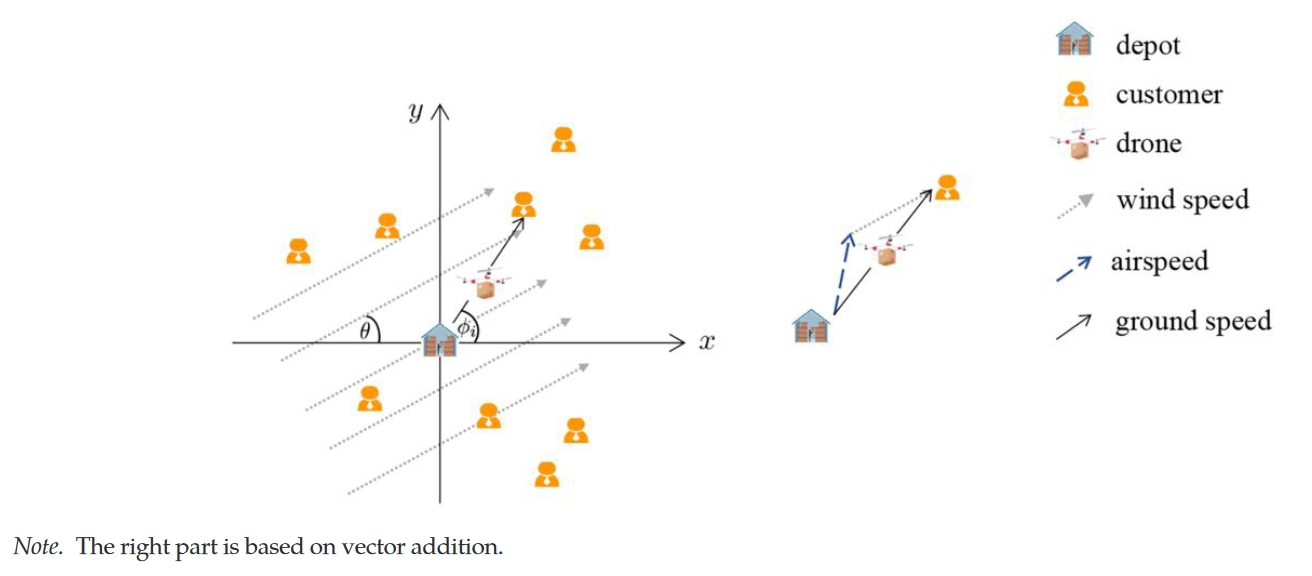
\includegraphics[width=0.7\linewidth]{figure_windspeed.png}
    \caption{Wind effect on the speed of drones by \cite{cheng2024robust}}
    \label{fig:WindEffect}
\end{figure}
where the airspeed denotes the speed of drones, and ground speed refers to the speed of drones relative to the ground. We assume that the calculation of speed is based on the vector addition. After the first-stage decision, at the beginning of the second-stage period, the wind condition is observed and remains constant throughout the time period $T$. Based on these assumptions, the time consumed by drones to finish a delivery can be calculated using following formulas proposed in \cite{cheng2024robust}:
\begin{equation}
    \begin{cases}
        t_f(v^{w}, \alpha^{w}) \triangleq \frac{d}{\sqrt{\left(v_f^{D}\right)^2 - \left(v^{w}\right)^2 \sin^2 \left( \alpha^{w} - \phi \right)} + v^{w} \cos \left( \alpha^{w}-\phi \right)} ,&\\
        t_b(v^{w}, \alpha^{w}) \triangleq \frac{d}{\sqrt{\left(v_b^{D}\right)^2 - \left(v^{w}\right)^2 \sin^2 \left( \alpha^{w} - \phi \right)} - v^{w} \cos \left( \alpha^{w}-\phi \right)} ,&
    \end{cases} \label{eq:time_wind}
\end{equation}
where the numerator of both equations are the distance between the depot/launch point and the gathering point. The notation $v_f^D$ denotes the airspeed of drone in the forward journey, and $v_b^D$ denotes the airspeed of drone in the backward journey. The angle $\phi$ is the angle between the depot/launch point and the gathering points, centering at the depot/launch point. With a pair of given wind condition $(v^{w}, \alpha^{w})$, the first equation calculates the forward time $t_f(v^{w}, \alpha^{w})$ consumed by drones from the depot/launch point to the gathering point, and the second equation derived the time consumed by drone returning from the gathering point, $t_b(v^{w}, \alpha^{w})$. 

In most drone delivery studies, the forward airspeed is assumed to be no larger than the backward airspeed, saying $v_f^D \leq v_b^D$. Because the airspeed of drones is correlated with the weight and size of the package it carrying. However, in this paper, we derive the average airspeed of drones based on the formula \ref{eq:range_speed_formula} proposed in \cite{dukkanci2021minimizing},
\begin{equation}
    R(v) \triangleq \frac{\Theta}{\frac{\mu_1}{v} + \mu_2 v + \frac{\mu_3}{v^2} + \mu_4 v^2}, \label{eq:range_speed_formula}
\end{equation}
where the range $R(v)$ (in m) of a drone traveling at a constant speed $v$ (in m/s). The parameters $\mu_1$, $\mu_2$, $\mu_3$, $\mu_4$, and $\Theta$ are constants that depend on the drone model, and the detailed calculation is listed in the \ref{app:drone_range}. This formula indicates that with a fully-charged battery, the maximum range a drone can achieve when flying at a constant speed $v$. We can calculate the average airspeed of drone by fixing the value of parameters $\mu_1$, $\mu_2$, $\mu_3$, $\mu_4$, $\Theta$ and setting the range $R = 2 \times d_{ij}$, where $d_{ij}$ is the distance between the gathering point $i$ and the depot/launch point $j$. To prevent deliveries in very windy conditions, we assume that if $v \leq v^{wind}$, a drone cannot be used to serve the gathering point $i$ from the depot/launch point $j$, which can be achieved by imposing the following constraints into the formulation \ref{formulation:2ndStage}:
\begin{subequations}
    \begin{align}
      x_{ilk} = 0, \quad &\forall i \in I, l \in \{L\cup D\}, k \in K_{SD}, \quad  \text{if} \quad v_{ilk} \leq v^{wind}, \label{constraint:SD_wind_speed_constraint} \\
      y_{idk} = 0, \quad &\forall i \in I, d \in D, k \in K_{LD}, \quad  \text{if} \quad v_{idk} \leq v^{wind}. \label{constraint:LD_wind_speed_constraint}
    \end{align}
\end{subequations}

After determining the maximum average airspeed $v_{max}$ of a drone for delivery from a depot/launch point to a gathering point,  if the drone is deemed suitable for the current gathering point, the total time taken by drones to complete the delivery can be calculated using formula \eqref{eq:range_speed_formula}, where we set $v_f^D = v_b^D = v_{max}$. 

\subsection{Sample Average Approximation} \label{subsec:SAA}
Stochastic programming is a powerful tool to solve optimization problems with uncertainties. However, the computational complexity of solving a two-stage stochastic programming problem with a continuous distribution is high. To address this issue, one typical approach is approximating the continuous distribution by finite discrete distributions, for example, using sample average approximation (SAA) (\cite{birge2011introduction}, \cite{kleywegt2002sample}). We assume that the supports of $\Xi$ is finite, which indicates that the demand, road distance and wind condition can take a finite number of values with positive probabilities. We can generate a large set of scenarios $S$, and the probability of each scenario is $\frac{1}{|S|}$. The SAA approximate the two-stage stochastic programming problem into a deterministic equivalent problem, which can be formulated as:
\footnotesize
\begin{subequations} \label{formulation:SAA}
    \begin{align}
        \min \quad & \frac{1}{|S|} \sum_{s \in S} \left(\sum_{i \in I} \pi o_{s,i} + \sum_{k \in K_{SD}} c_{SD} g_{s,k} + \sum_{k \in K_{LD}} c_{LD} g_{s,k} \right) && \label{objective:SAAObj} \\
        \subjectto \quad & \text{Constraints (\ref{constraint:Num_Depot}) - (\ref{constraint:vBinary})} && \label{constraint:1stStage_SAA}\\
                        & \text{Constraints \eqref{constraint:SD_wind_speed_constraint} - \eqref{constraint:LD_wind_speed_constraint}} && \label{constraint:wind_speed}\\
                        & y_{sidk} \leq u_d && \forall s \in S , d \in D, i \in I, k \in K_{LD} \label{constraint:DepotOpen1_SAA}\\
                        & x_{silk} \leq u_l && \forall s \in S , l \in D, i \in I, k \in K_{SD} \label{constraint:DepotOpen2_SAA}\\
                        & x_{silk} \leq v_l && \forall s \in S , l \in L, i \in I, k \in K_{SD} \label{constraint:LaunchPointOpen_SAA} \\
                        & \sum_{i \in I} \sum_{l \in \{L \cup D\}} x_{silk} \leq g_{s,k} && \forall s \in S , k \in K_{SD} \label{constraint:SmallDrone_Usage_SAA}\\
                        & \sum_{i \in I} \sum_{d \in D}y_{sidk} \leq g_{s,k} && \forall s \in S , k \in K_{LD} \label{constraint:LargeDrone_Usage_SAA}\\
                        & \sum_{k \in K_{SD}} \sum_{i \in I} q_{s,i} x_{silk} \leq Q_T v_l && \forall s \in S , l \in L \label{constraint:TrucksCapacity_SAA} \\
                        & q_{s,i} - \sum_{k \in K_{SD}}\sum_{l \in \{L \cup D\}} Q_{SD} x_{silk} - \sum_{k \in K_{LD}}\sum_{d \in D} Q_{LD} y_{sidk} \leq o_{s,i} && \forall s \in S , i \in I \label{constraint:UnmetDemand_SAA} \\
                        & \sum_{d \in D} \frac{\omega_{sld}}{v_T} w_{ld} + \sum_{i \in I} \left( \frac{2d_{li}}{v_{sli}} + \tau \right) x_{silk} \leq T && s \in S , \forall l \in L, k \in K_{SD} \label{constraint:LPTimeLimitSD_SAA} \\
                        & \sum_{i \in I} \left( \frac{2d_{li}}{v_{sli}} + \tau \right) x_{silk} \leq T && \forall s \in S , l \in D, k \in K_{SD} \label{constraint:DepotTimeLimitSD_SAA} \\
                        & \frac{2d_{ji}}{v_{sji}} y_{sijk} \leq T && \forall s \in S , j \in D, i \in I, k \in K_{LD} \label{constraint:DepotTimeLimitLD_SAA} \\
                        & g_{s,k} \geq g_{s,k+1} && \forall s \in S , k, k+1 \in K_{SD} \label{constraint:SD_Remove_Symmetry_SAA} \\
                        & g_{s,k} \geq g_{s,k+1} && \forall s \in S , k, k+1 \in K_{LD} \label{constraint:LD_Remove_Symmetry_SAA} \\
                         & g_{s,k} \in \{0,1\}, && \forall s \in S , k \in \{K_{SD} \cup K_{LD}\} \label{constraint:gBinary_SAA} \\
                         & x_{silk} \in \{0,1\}, && \forall s \in S , l \in L, i \in I, k \in K_{SD} \label{constraint:xBinary_SAA} \\
                         & y_{sidk} \in \{0,1\}, && \forall s \in S , d \in D, i \in I, k \in K_{LD} \label{constraint:yBinary_SAA} \\
                         & o_si \geq 0, && \forall  s \in S , i \in I \label{constraint:Unmet}
    \end{align}
\end{subequations}
\normalsize

\section{Solution Strategies}\label{sec:methods}
In this section, we will introduce two solution strategies to solve the SAA formulation. The first strategy is the scenario decomposition algorithm (SDA), which is proposed by \cite{ahmed2013SDA} for two-stage 0-1 stochastic programs where the first-stage decisions are binary. The second strategy is using a cluster-based heuristic algorithm to solve the first-stage decision variables as a warm start, then solving the second-stage problem by fixing the value of the first-stage decision variables. 

\subsection{Scenario Decomposition Algorithm} \label{subsec:SDA}
The scenario decomposition algorithm (SDA) is a decomposition algorithm that solves two-stage stochastic programming problems with binary first-stage decisions. In stochastic programming, one important implicit constraint for the first-stage problem is the nonanticipativity constraint, which requires that the first-stage decision must be independent of the realization of the random variable. The Scenario Decomposition Algorithm (SDA) comprises two phases. During the first phase, the nonanticipativity of the first-stage decision variables is relaxed. This relaxation enables the decomposition of the problem into individual scenarios. Each scenario is treated as a deterministic problem, and solving these yields a lower bound for the main problem based on the optimal values from the single-scenario problems. In the second phase, the algorithm fixes the first-stage decision variables using the solutions obtained in the first phase and solves for an upper bound for each scenario. Consequently, the upper bound for the main problem is derived by considering the expected value of the single-scenario solutions. Furthermore, the algorithm excludes the already evaluated first-stage variables in subsequent iterations and identifies tight lower bounds in the first phase. Given that the first-stage decision variables are binary, the following constraint can be added to the formulation to exclude previously evaluated solutions and establish a tight lower bound:
\begin{subequations} 
    \begin{align*}
        & \sum_{j \in D: \bar{x}_j = 0} \bar{x}_j + \sum_{j \in D: \bar{x}_j = 1} (1 - \bar{x}_j) + \sum_{l \in L: \bar{y}_l = 0} \bar{y}_l + \sum_{l \in L: \bar{y}_l = 1} (1 - \bar{y}_l) \\ \label{constraint:remove_tested_sol} \tag{7}
        & + \sum_{l \in L, j \in D: \bar{w}_{lj} = 0} \bar{w}_{lj} + \sum_{l \in L, j \in D: \bar{w}_{lj} = 1} (1 - \bar{w}_{lj}) \geq 1 \quad \forall \{\bar{x}, \bar{y}, \bar{w}\} \in R
    \end{align*}
\end{subequations}
where $R$ represents the set of first-stage variable solutions that have already been evaluated. A pseudocode representation of the SDA algorithm is provided in Algorithm \ref{alg:SDA}. The algorithm will conclude after a finite number of iterations, either by identifying infeasibility or by finding the optimal solution to the problem.The algorithm guarantees finding the optimal solution because any unexplored first-stage solution cannot yield a better objective value than $UB$, given that $UB \leq LB$. Therefore, $\{x^*, y^*, w^*\}$ represents the optimal solution to the problem.

\begin{algorithm}[h]
    \caption{Scenario decomposition algorithm} \label{alg:SDA}
    \begin{algorithmic}[1]
    \State \textbf{initialize:} $UB \gets +\infty, LB \gets -\infty, R \gets \emptyset, x^* \gets 0, y^* \gets 0, w^* \gets 0$
    \While {$UB > LB$ and $\{0,1\}^{(D+L+DL)} \setminus R \neq \emptyset$}
        \For {$s = 1$ to $S$}
            \State solve the \textit{relaxation} of the second stage formulation including constraints (\ref{constraint:remove_tested_sol})
            \State let $(\bar{x}_s, \bar{y}_s, \bar{w}_s)$ be the optimal solution and $lb_s$ be the optimal objective value
        \EndFor
        \State $LB \gets \sum_{s=1}^S p_s lb_s$, $\hat{R} \gets \bigcup_{s=1}^S \{\bar{x}_s, \bar{y}_s, \bar{w}_s\}$, $R \gets R \cup \hat{R}$
        \For {$\{x, y, w\} \in \hat{R}$}
            \State $u \gets 0$
            \For {$s = 1$ to $S$}
                \State solve the problem formulation given $x, y,$ and $w$ variables
                \State let $f_s(x, y, w)$ be the optimal objective value
                \If {Problem is infeasible}
                    \State set $f_s(x, y, w) \gets \infty$ and $u \gets \infty$
                \Else
                    \State set $u \gets u + p_s f_s(x, y, w)$
                \EndIf
            \EndFor
            \If {$UB > u$}
                \State $UB \gets u, x^* \gets x, y^* \gets y$ and $w^* \gets w$
            \EndIf
        \EndFor
    \EndWhile
    \end{algorithmic}
\end{algorithm}
Similar to the preprocessing in \cite{dukkanci2023drones}, in the scenario algorithm phase of the algorithm where the $UB$ is evaluated, according to the constraints \eqref{constraint:DepotOpen1_SAA}, \eqref{constraint:DepotOpen2_SAA}, and \eqref{constraint:LaunchPointOpen_SAA}, if the first-stage decision variables $u_d = 0, \forall d \in D$ or $v_l = 0, \forall l \in L$, the corresponding second-stage decision variables $y_{sidk}$ and $x_{silk}$ will not be defined.

\subsection{Cluster-based Heuristic Algorithm} \label{subsec:Cluster_Heuristic}
The SAA formulation \ref{formulation:SAA} is usually difficult to solve when the number of scenarios is large. However, if the value of the first-stage decision variables are fixed, the remaining work is solving the second-stage problems iteratively, which is a relatively easy task compared to solving the entire SAA formulation all at once. The SDA is built based on this idea (from line 3 to 6 in algorithm \ref{alg:SDA}), whereas at the beginning of the SDA algorithm, the ``quality'' of its first-stage solutions cannot be guaranteed. Therefore, in most cases, the performance of SDA would take a lot of iterations before it converges. Facing this challenge, we want to find good value first-stage variable within a short time, and consequently we propose the cluster-based heuristic algorithm. 

In our problem, one key property is that the objective function completely depends on the second-stage decision variables, specifically the summation of the penalty for unmet demands and the cost of using drones. However, as mentioned earlier, the range limit of drones and the time window restriction determine whether a gathering point can be covered by drones. Therefore, the location of drone facilities is crucial, and the value of the first-stage decision variables implicitly affects the objective function. Although all potential locations for the drone facilities are predetermined, and some road networks may be disrupted after the earthquake, the aerial distance between locations remains unchanged. Based on the assumption made in Section \ref{sec:formulation}, there are more open launch points than open depots. Therefore, we prioritize the distance between open launch points and gathering points over the distance between open depots and gathering points. The complete steps of the cluster-based heuristic algorithm are shown as follows:
\setlist[enumerate,1]{label=Step \arabic*., leftmargin=*, labelwidth=4em, topsep=0em, itemsep=0em, parsep=0em}
\begin{enumerate}[itemsep=0em]
    \item Using $k$-means algorithm to cluster the gathering points into $p$ clusters, where $p$ is the maximal number of open launch points;
    \item For each launch point, calculate the total distance between the launch point and all gathering points in a certain cluster and assign the launch points to the certain cluster of gathering points with smallest the total distance;
    \item Among all the launch points assigned to the same cluster, select the launch point with the smallest total distance to the gathering points in the cluster as the open launch point;
    \item Using $k$-means algorithm to cluster all the open launch points into $e$ clusters, where $e$ is the maximal number of open depots;
    \item For each depot, calculate the total distance between the depot and all open launch points in a certain cluster and the total distance between the depot and all the gathering points assigned to those launch points. Assign the depots to the certain cluster of launch points with smallest the total distance;
    \item Among all the depots assigned to the same cluster of launch points, select the depot with the smallest total distance to the open launch points in the cluster as the open depot, the remains are closed.
    \item The value of the first-stage decision variables $u_d$ and $v_l$ are determined by the open depots and launch points, and the assignment of launch points to depots is determined in Step 6.
    \item Fix the value of the first-stage decision variables and solve the second-stage problem in each scenario. Take the average of the objective value of all scenarios as the objective value of the optimal solution.
\end{enumerate}

\subsection{Benders Decomposition in Mixed-Integer Programming (MIP)} \label{subsec:Benders_MIP}
Benders decomposition was first proposed to solve large-scale linear programming problems, which is also a common technique to solve the two-stage stochastic programming problems. A brief recap of Benders decomposition can be found in \ref{app:Benders_Recap}. Nevertheless, Benders decomposition can not be directly applied to the mixed-integer programming problem. In the original Benders decomposition, the dual variables are required to generate both feasibility cuts and optimality cuts. However, in the mixed-integer programming, the dual variables are not well-defined for those constraints containing integer variables. 

For stochastic integer programs with binary first-stage decision variable, there are only a finite number of feasible first stage solutions. Let $ r = 1 \dots R$, index these feasible solutions and $x$ refer to the $r$-th feasible solution. One integer optimality cut was proposed in \cite{laporte1993integer} as follows:
\begin{align}
    \theta \geq \left( Q_{r}(x) - L \right) \left( \sum_{i \in S_r} x_i - \sum_{i \notin S_r} x_i \right) - \left( Q_{r}(x) - L \right) (|S_r| - 1) + L, \label{eq:integer_benders_cut} 
\end{align}
where $x_i = 1, \forall i \in S_r$, $x_i = 0, \forall i \notin S_r$. $Q_r(x)$ is the corresponding expected second-stage value. Notation $|S_r|$ refers to the cardinality of the $S_r$. The $L$ is the lower bound of the second-stage objective function, which can be calculated by solving the LP relaxation. The $\theta$ is an auxiliary variable introduced to approximate the value of $Q(x)$, and the resulting master problem is shown following:
\begin{subequations} 
    \begin{align*}
              \min \quad & c^T x + \theta \\
        \subjectto \quad & Ax = b  \\
                         \theta \geq & \left( Q_{r}(x) - L \right) \left( \sum_{i \in S_r} x_i - \sum_{i \notin S_r} x_i \right) - \left( Q_{r}(x) - L \right) (|S_r| - 1) + L, \quad r = 1 \dots R\\
                         & x \in \Zmbb^n_+, \theta \in \Rmbb,
    \end{align*}
\end{subequations}
where we assume that such stochastic programming problem has complete recourse, which means for every solution to the first-stage problem, the second-stage problem is always feasible. The cut (\ref{eq:integer_benders_cut}) is a valid cut for the problem incident with integer decision variables, which can be used to provide a lower bound of the objective function in a pure-integer case.

However, the cut (\ref{eq:integer_benders_cut}) is not tight when the second-stage problem is formulated as a MIP. Therefore, simply applying the cut (\ref{eq:integer_benders_cut}) to our problem cannot guarantee a good solution. So far, to the best of our knowledge, there is only one existing literature that provides a converging Bender decomposition algorithm for the mixed-integer programming problem, which is proposed by \cite{van2023converging}. Nevertheless, due the limited time and the complexity of the algorithm, we will not implement this algorithm in our study and Benders decomposition will not be considered in the numerical experiments as a comparison.

\section{Computational Results}\label{sec:results}
This section provides a comprehensive analysis of the computational experiments conducted in this study. Firstly, we describe the datasets used. Secondly, we explain the calculation of road distance values under different earthquake scenarios. Thirdly, we evaluate the performance of the SDA, the heuristic algorithm, and the values of stochasticity and perfect information. Finally, we conduct a thorough analysis of the fairness problem.

All the mathematical algorithms are implemented in Python, and all the experiments are implemented in the Windows environment with an Intel Core i7-13700 CPU and 64 GB of RAM. The optimization problems are solved using the Gurobi Optimizer 9.1.2. The source code of the implementation can be found in the supplementary material.

\subsection{Dataset} \label{subsec:Dataset}
With the fact that the detailed realistic data is not available, we generate the dataset using the random function in Python. The dataset is built on a $300 \times 300$ grid, where we assume each unit distance is 1 kilometer in the real world. According to the problem's statement, the locations of gathering points, and potential locations of launch points and depots are predetermined. Therefore, we use random function to generate 25 candidate locations for launch points and 10 candidate locations for depots. The number of gathering points is 40, the same as the number used in \cite{dukkanci2023drones}. The locations generated above are non-overlapping and fixed throughout different scenarios. 

After determining the fixed locations for facilities, the value of uncertain parameters needs to be considered. In every series of tests, there are 12 different scenarios, which also refers to the values used in \cite{dukkanci2023drones}. For the uncertain wind condition, we generate the speed (in km/hr) using the distribution U$(0,20)$. The value is set in this way based on the location data generated before, so that the wind won't be too strong that no drones can deliver relief items. The direction of wind is generated with the distribution U$(0,2\pi)$. Compared to the way of calculating the demand at each gathering point in \cite{dukkanci2023drones}, we generate the demand (in kg) at each gathering point in a simpler way, using the distribution U$(0.02,20)$. The range of demand value is based on the data provided in \cite{dukkanci2023drones}. The value of the earthquake information will be demonstrated in the next section.

\subsection{Road Distance after Earthquake} \label{subsec:RoadDistance}
To assess the impact of the earthquake on each facility location, we need to calculate the earthquake intensity. In the field of geology, various predictive models have been proposed and evaluated to determine the Medvedev Sponheuer Karnik (MSK) scale, which indicates the level of damage intensity ($I_s$). The MSK scale is a 12-point scale, and the intensity of the earthquake is determined by the distance between the epicenter and the facility location $R_{epi}$, the surface-wave magnitude ($M_s$) and the hypocentral depth of the earthquake $h$. As studied in recent work \cite{erbeyouglu2020earthquake}, they evaluated four intensity predictive models that can be applied to estimate the damage for all potential earthquakes:
\begin{subequations}
    \begin{align}
    I_s &= 7.023 + 0.703 M_s - 2.826  \log_{10}(R_{epi}), \label{eq:MSK_1} \\
    I_s &= 5.002 + 0.75 M_s - 0.0094  R_{epi} - 1.454 \log_{10}(R_{epi}) \label{eq:MSK_2}, \\
    I_s &= 7.494 + 0.744 M_s - 3.377 \log_{10} \sqrt[3]{R_{epi}^3 + h^3} + 0.017 h \label{eq:MSK_3}, \\
    I_s &= 2.281 + 0.874 M_s - 0.618 \log_{10} \sqrt{1+\frac{R_{epi}^2}{h^2}} - 0.016 \left(\sqrt{h^2 + R_{epi}^2} - h\right) \label{eq:MSK_4}.
    \end{align}
\end{subequations}

After the earthquake, the distance between the epicenter and each facility location can be computed. With the known magnitude and hypocentral depth of the earthquake, the intensities of the earthquake can be calculated by formulas (\ref{eq:MSK_1}) - (\ref{eq:MSK_4}). In \cite{erbeyouglu2020earthquake}, they did not indicate the best formula among \eqref{eq:MSK_1} - \eqref{eq:MSK_4} for estimating the damage intensity. The average of the intensity values from the four formulas is used as the final intensity value for a certain facility. According to the MSK value, we can estimate how severe the damage is at each facility location using figure \ref*{fig:MSK_scale}.
\begin{figure}
    \centering
    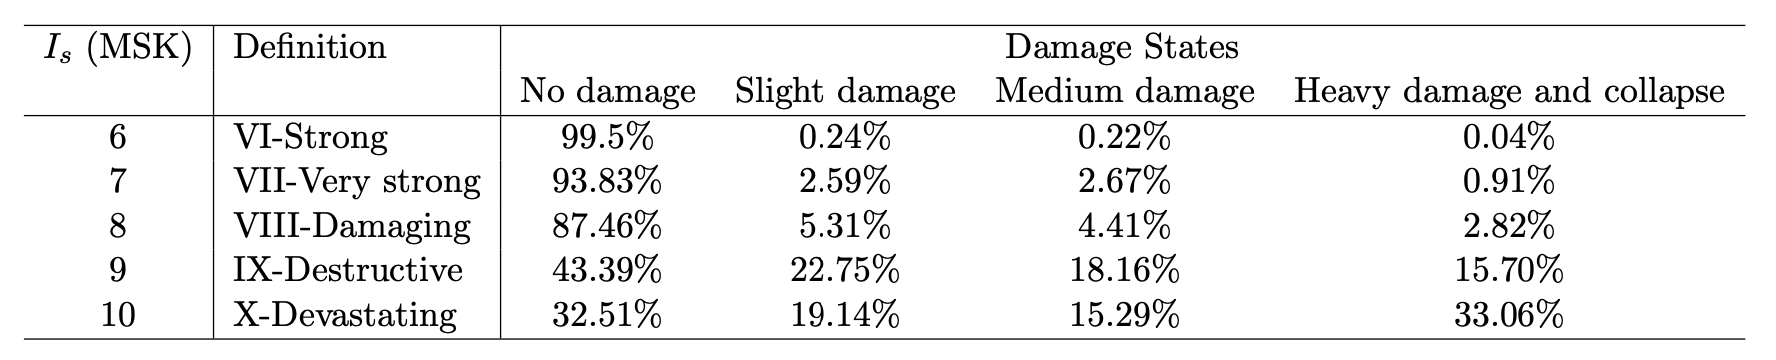
\includegraphics[width=\textwidth]{eq_tab.png}
    \label{fig:MSK_scale}
    \caption{Damage percentages based on 1999 Izmit Earthquake (\cite{ozmen2002istanbul})}
\end{figure}

For determining the road distance, we calculate the damage percentages of the depot and launch points and consider their average. We subsequently increase the road distance by the average. In experiments, for each one of the 12 scenarios, we use the same value for the magnitude and depth of the earthquake in \cite{dukkanci2023drones}:
\begin{table}[h]
    \centering
    \caption{Magnitude and Depth values (\cite{dukkanci2023drones})}
    \begin{tabular}{|c|c|c|c|c|c|c|c|c|c|c|c|c|}
    \hline
    & 1 & 2 & 3 & 4 & 5 & 6 & 7 & 8 & 9 & 10 & 11 & 12 \\
    \hline
    Magnitude & 7.5 & 6.8 & 7.7 & 7.6 & 7.7 & 6.8 & 7.3 & 7.0 & 6.8 & 7.7 & 6.8 & 7.7 \\
    \hline
    Depth & 5.3 & 14.4 & 5.4 & 16 & 12.7 & 8.7 & 12.6 & 8.2 & 12.7 & 12.7 & 16.9 & 8.7 \\
    \hline
    \end{tabular}
    \label{tab:earthquake_info}
\end{table}
For the setting of other parameters, we set the speed of truck $v_T$ as $45$ km/hr, capacity of truck $Q_T$ to be 2000 kg. The maximum speed limit for drones traveling between launch point/depots and gathering point is calculated using the range function given in equation \eqref{eq:range_speed_formula}. To ensure that all deliveries are completed within a reasonable time, the time-bound $T$ is set as 2.5 hours. More detailed information about drones' parameter is listed in \ref{app:drone_range}.

\subsection{Results Analysis} \label{subsec:test_results}
\subsubsection{Performance Evaluation} \label{subsubsec:performance_eval}
In this section, we conduct numerical experiments to evaluate the performance of the SDA and heuristic algorithm. We set the maximum number of open launch points to be 4, 5, and 6, and the maximum number of open depots to be 1 and 2. We combine the number of available drones of each type together, resulting in 3 kinds of bundles: 10 small drones and 1 large drone, 15 small drones and 2 large drones, and 20 small drones and 3 large drones. The numerical test results are shown in Table \ref{tab:performance}. The column ``SAA'' stands for results directly solved by the Gurobi solver, the column ``SDA'' refers to results obtained by the scenario decomposition algorithm, and the column ``Heuristic'' states results obtained by the cluster-based heuristic algorithm. From the results, we can tell that our problem formulation is not complicated, and the Gurobi solver with default settings can solve the problem fast. In this case, the poor performance of SDA in terms of time can be well-explained. Even though the SDA gets the optimal solution, it takes many iterations to converge as reflected by the running time. Compared to the outstanding performance shown in \cite{dukkanci2023drones}, we may conclude that SDA only has advantages when the dataset is very large, and the number of scenarios is not many. The heuristic algorithm, on the other hand, shows a good performance in terms of both time and solution quality. The gap between the heuristic algorithm and the optimal solution is less than 5\% in most cases, which is acceptable in practice. At the same time, it is the fastest algorithm compared to the other two.

\begin{table}[!h]\centering
    \caption{Performance of the proposed algorithms}\label{tab:performance} \resizebox{\textwidth}{!}{
    \begin{tabular}{|c|cccc|cc|cc|ccc|} 
        \hline
            Series & $p$ & $e$ & $K_{SD}$ & $K_{LD}$ & SAA & Time (s) & SDA & Time (s) & Heuristic & Time (s) & Gap (\%) \\
            \hline
            1 & 4 & 1 & 10 & 1 & 4038.84 & 8.64 & 4038.84 & 116.76 & 4201.05 & 8.48 & 4.02 \\
            1 & 4 & 1 & 15 & 2 & 3921.66 & 13.12 & 3921.66 & 175.12 & 4116.05 & 12.77 & 4.96 \\
            1 & 4 & 1 & 20 & 3 & 3851.17 & 17.27 & 3850.83 & 243.13 & 4031.05 & 16.99 & 4.67 \\
            1 & 4 & 2 & 10 & 1 & 4036.47 & 9.51 & 4036.47 & 130.9 & 4073.26 & 8.38 & 0.91 \\
            1 & 4 & 2 & 15 & 2 & 3806.17 & 15.29 & 3806.17 & 200.29 & 3967.86 & 12.65 & 4.25 \\
            1 & 4 & 2 & 20 & 3 & 3686.25 & 20.46 & 3686.25 & 268.38 & 4022.40 & 16.85 & 9.12 \\
            1 & 5 & 1 & 10 & 1 & 4038.84 & 9.93 & 4038.84 & 135.04 & 4201.05 & 8.54 & 4.02 \\
            1 & 5 & 1 & 15 & 2 & 3921.66 & 15.09 & 3921.66 & 202.01 & 4164.75 & 12.9 & 6.20 \\
            1 & 5 & 1 & 20 & 3 & 3851.17 & 20.21 & 3850.83 & 268.94 & 4031.05 & 16.96 & 4.67 \\
            1 & 5 & 2 & 10 & 1 & 4036.47 & 9.6 & 4036.47 & 127.77 & 4208.28 & 8.56 & 4.26 \\
            1 & 5 & 2 & 15 & 2 & 3806.17 & 14.14 & 3806.17 & 200.91 & 3912.02 & 13.04 & 2.78 \\
            1 & 5 & 2 & 20 & 3 & 3686.25 & 20.98 & 3686.25 & 269.32 & 4072.72 & 17.41 & 10.48 \\
            1 & 6 & 1 & 10 & 1 & 4038.84 & 9.99 & 4038.84 & 134.67 & 4201.05 & 8.47 & 4.02 \\
            1 & 6 & 1 & 15 & 2 & 3921.66 & 15.35 & 3921.66 & 201.78 & 4116.05 & 12.69 & 4.96 \\
            1 & 6 & 1 & 20 & 3 & 3851.17 & 20.55 & 3850.83 & 270.05 & 4031.05 & 16.97 & 4.67 \\
            1 & 6 & 2 & 10 & 1 & 4036.47 & 9.81 & 4036.47 & 135.14 & 4051.09 & 8.47 & 0.36 \\
            1 & 6 & 2 & 15 & 2 & 3806.17 & 14.88 & 3806.17 & 196.79 & 3911.91 & 12.71 & 2.78 \\
            1 & 6 & 2 & 20 & 3 & 3686.25 & 18.9 & 3686.25 & 270.72 & 3837.35 & 17.25 & 4.10 \\
            \hline
            \multicolumn{5}{|c|}{Series 1 Average} & & 14.65 & & 197.10 & & 12.78 & 4.51 \\
            \hline
            2 & 4 & 1 & 10 & 1 & 4245.84 & 9.93 & 4245.84 & 135.17 & 4384.53 & 8.53 & 3.27 \\
            2 & 4 & 1 & 15 & 2 & 4069.13 & 14.70 & 4069.13 & 203.39 & 4299.53 & 12.96 & 5.66 \\
            2 & 4 & 1 & 20 & 3 & 3992.93 & 20.06 & 3992.93 & 271.61 & 4218.23 & 16.91 & 5.64 \\
            2 & 4 & 2 & 10 & 1 & 4213.61 & 10.03 & 4213.61 & 135.46 & 4365.55 & 8.49 & 3.61 \\
            2 & 4 & 2 & 15 & 2 & 4008.26 & 14.91 & 4008.26 & 204.19 & 4069.13 & 12.79 & 1.52 \\
            2 & 4 & 2 & 20 & 3 & 3839.92 & 20.31 & 3839.92 & 273.11 & 4367.98 & 17.06 & 13.76 \\
            2 & 5 & 1 & 10 & 1 & 4245.84 & 10.01 & 4245.84 & 133.91 & 4384.53 & 8.52 & 3.27 \\
            2 & 5 & 1 & 15 & 2 & 4069.13 & 12.98 & 4069.13 & 467.54 & 4299.53 & 12.71 & 5.66 \\
            2 & 5 & 1 & 20 & 3 & 3992.93 & 21.09 & 3992.93 & 242.95 & 4214.53 & 16.78 & 5.56 \\
            2 & 5 & 2 & 10 & 1 & 4213.61 & 8.61 & 4213.61 & 123.31 & 4245.84 & 8.46 & 0.76 \\
            2 & 5 & 2 & 15 & 2 & 4008.26 & 13.40 & 4008.26 & 190.57 & 4389.05 & 12.55 & 9.50 \\
            2 & 5 & 2 & 20 & 3 & 3839.92 & 17.88 & 3839.92 & 246.48 & 3992.93 & 16.97 & 3.99 \\
            2 & 6 & 1 & 10 & 1 & 4245.84 & 9.26 & 4245.84 & 119.70 & 4245.84 & 8.49 & 0.00 \\
            2 & 6 & 1 & 15 & 2 & 4069.13 & 13.13 & 4069.13 & 175.79 & 4299.53 & 12.64 & 5.66 \\
            2 & 6 & 1 & 20 & 3 & 3992.93 & 17.38 & 3992.93 & 234.58 & 4218.23 & 16.73 & 5.64 \\
            2 & 6 & 2 & 10 & 1 & 4213.61 & 8.40 & 4213.61 & 115.31 & 4245.84 & 8.40 & 0.76 \\
            2 & 6 & 2 & 15 & 2 & 4008.26 & 12.75 & 4008.26 & 175.50 & 4069.13 & 12.75 & 1.52 \\
            2 & 6 & 2 & 20 & 3 & 3839.92 & 17.26 & 3839.92 & 234.47 & 3984.13 & 17.07 & 3.76 \\
            \hline
            \multicolumn{5}{|c|}{Series 2 Average} & & 13.92 & & 197.23 & & 12.97 & 4.07 \\
            \hline
    \end{tabular}}
\end{table}

% \begin{table}[!h]\centering
%     \caption{Performance of the proposed algorithms Cont.} \label{tab:performance_cont}
%     \resizebox{\textwidth}{!}{
%     \begin{tabular}{|c|cccc|cc|cc|ccc|}
%         \hline
%             Serie& $p$ & $e$ & $K_{SD}$ & $K_{LD}$ & SAA & Time (s) & SDA & Time (s) & Heuristic & Time (s) & Gap (\%) \\
%             \hline
%             3 & 4 & 1 & 10 & 1 & 3159.28 & 8.55 & 3159.28 & 116.57 & 3330.20 & 8.40 & 5.41 \\
%             3 & 4 & 1 & 15 & 2 & 3046.23 & 13.12 & 3046.23 & 174.33 & 3267.43 & 12.80 & 7.27 \\
%             3 & 4 & 1 & 20 & 3 & 3046.23 & 17.37 & 3046.23 & 233.16 & 3241.61 & 16.83 & 6.41 \\
%             3 & 4 & 2 & 10 & 1 & 3156.06 & 8.44 & 3156.06 & 115.85 & 3404.05 & 8.44 & 7.86 \\
%             3 & 4 & 2 & 15 & 2 & 2964.37 & 12.76 & 2964.37 & 173.91 & 3239.77 & 12.69 & 9.27 \\
%             3 & 4 & 2 & 20 & 3 & 2898.28 & 17.12 & 2898.08 & 232.30 & 3155.16 & 16.98 & 8.87 \\
%             3 & 5 & 1 & 10 & 1 & 3159.28 & 8.56 & 3159.28 & 116.61 & 3324.77 & 8.46 & 5.24 \\
%             3 & 5 & 1 & 15 & 2 & 3046.23 & 13.02 & 3046.23 & 174.20 & 3266.84 & 12.66 & 7.25 \\
%             3 & 5 & 1 & 20 & 3 & 3046.23 & 17.41 & 3046.23 & 233.21 & 3224.91 & 17.10 & 5.87 \\
%             3 & 5 & 2 & 10 & 1 & 3156.06 & 8.53 & 3156.06 & 115.88 & 3467.39 & 8.50 & 9.86 \\
%             3 & 5 & 2 & 15 & 2 & 2964.37 & 12.90 & 2964.37 & 173.85 & 3415.05 & 12.68 & 15.21 \\
%             3 & 5 & 2 & 20 & 3 & 2898.28 & 17.15 & 2898.08 & 232.60 & 3268.26 & 16.77 & 12.75 \\
%             3 & 6 & 1 & 10 & 1 & 3159.28 & 8.52 & 3159.28 & 116.16 & 3324.77 & 8.42 & 5.24 \\
%             3 & 6 & 1 & 15 & 2 & 3046.23 & 12.87 & 3046.23 & 174.22 & 3239.77 & 12.80 & 6.35 \\
%             3 & 6 & 1 & 20 & 3 & 3046.23 & 17.46 & 3046.23 & 233.18 & 3154.77 & 16.91 & 3.56 \\
%             3 & 6 & 2 & 10 & 1 & 3156.06 & 8.48 & 3156.06 & 115.88 & 3155.70 & 8.38 & -0.01 \\
%             3 & 6 & 2 & 15 & 2 & 2964.37 & 12.94 & 2964.37 & 173.21 & 3467.39 & 12.49 & 16.95 \\
%             3 & 6 & 2 & 20 & 3 & 2898.28 & 17.26 & 2898.08 & 232.32 & 3154.77 & 16.90 & 8.85 \\
%             \hline
%             \multicolumn{5}{|c|}{Series 3 Average} & & 12.73 & & 181.30 & & 12.90 & 7.79 \\
%             \hline
%     \end{tabular}}
% \end{table}
\subsubsection{Large Number Scenarios} \label{subsubsec:large_scenarios}
In this test, we fixed the maximal number of open launch points to be 10 and the maximal number of open depots to be 4. We set the number of small drones to be 20 and the number of large drones to be 3. We increase the number of scenarios to 20, 50, and 100. The results are shown in Table \ref{tab:large_scenario}. The result confirms our assumptions that the SDA algorithm is not suitable for the large number of scenarios. The running time of the SDA algorithm increases exponentially with the number of scenarios. The heuristic algorithm, on the other hand, shows a good performance in terms of both time and solution quality. 

\begin{table}[!htp]\centering
    \caption{Test on Large Number of S}\label{tab:large_scenario}
    \scriptsize
    \begin{tabular}{|c|c|cccc|cc|cc|cc|}
    \hline
    Test &$S$ &$p$ &$e$ &$K_{SD}$ &$K_{LD}$ &Heuristic &Time (s) &SAA &Time (s) &SDA &Time (s) \\
    \hline
    7 &20 &10 &4 &20 &3 &4054.92 &28.63 &4004.85 &30.99 &4004.85 &741.87 \\
    8 &50 &10 &4 &20 &3 &3257.99 &71.53 &3217.14 &76.65 &3217.14 &4945.52 \\
    9 &100 &10 &4 &20 &3 &3728.52 &147.82 &3428.72 &158.42 &3428.69 &16002.26 \\
    \hline
    \end{tabular}
\end{table}

\subsubsection{Value of Stochasticity and Perfect Information} \label{subsubsec:stochasticity}
In this section, a test is conducted to evaluate the value of considering the uncertain wind conditions. We fix the maximal number of open launch point to be 10, and maximal number of open depots is 4. The number of available small drone and large drones are set to be 30 and 5, respectively. We first formulate the model in \cite{dukkanci2023drones}, and solve it on our dataset to retrieve the first-stage decisions. Our SAA model is also resolved on the same dataset, and result indicates for the original model, the objective function value is 3018.54 while our model has the objective value as 3400.84. This result matches our expectation, since the original model does not consider the uncertain wind condition. It leads to an ideal scenario that no delivering process will be affected by uncertain conditions. 
\begin{table}[!htp]
    \centering
    \caption{Scenario Analysis with New Model and Original Model}
    \resizebox{0.6\textwidth}{!}{
    \begin{tabular}{|ccccc|}
    \hline
    Scenario & Our Model & $o_s$ & Original Model & $o_s$ \\
    \hline
    1 & 3336.42 & 7.97 & 3861.05 & 9.43 \\
    2 & 3336.42 & 7.97 & 3861.05 & 9.43 \\
    3 & 3336.42 & 7.97 & 3861.05 & 9.43 \\
    4 & 3445.20 & 8.28 & 3927.27 & 9.62 \\
    5 & 3445.20 & 8.28 & 3927.27 & 9.62 \\
    6 & 3336.42 & 7.97 & 3861.05 & 9.43 \\
    7 & 3553.75 & 8.61 & 4079.85 & 10.06 \\
    8 & 3336.42 & 7.97 & 3861.05 & 9.43 \\
    9 & 3336.42 & 7.97 & 3861.05 & 9.43 \\
    10 & 3337.78 & 7.97 & 3861.05 & 9.43 \\
    11 & 3445.20 & 8.28 & 3927.27 & 9.62 \\
    12 & 3564.49 & 8.64 & 4079.85 & 10.06 \\
    \hline
    Average & 3400.85 & 8.15 & 3914.07 & 9.58 \\
    \hline
    \end{tabular}}
    \label{tab:scenario_analysis}
\end{table}

After fixing the value of first-stage decisions retrieved from both new model and original model, the problem is solved in 12 different scenarios separately. The test result is illustrated in the table \ref{tab:scenario_analysis}. The column ``Our Model'' stands for to the objective value of the new model, and the column ``$o_s$'' refers to the value of the unmet demand in the second stage calculated by the new model. The column ``Original Model'' represents to the objective value of the original model, and the column ``$o_s$'' refers to unmet demand in the second stage calculated by the original model. The test result shows perfectly how significant is to consider the uncertain weather conditions, lower objective value and lower average unmet demand. 

Moreover, in this specific test, the value of stochasticity (VS) is: $\frac{z_{old} - z_{new}}{z_{new}} \approx 0.151$, where $z_{old}$ refers to the average objective value of original model, and $z_{new}$ represents the average objective value of our model. The expected value of perfect information (EVPI) is calculated as by $\frac{z_{new} - z_{perfect}}{z_{new}}$, where $z_{perfect}$ is the expectation of the objective value in different scenarios, which can be easily calculated by solving each scenario separately, then taking the expectation of all the results. We do not show the evaluation process in this study, since the dataset we test on is rare that first-stage decisions are the same in all scenarios, which is same as the solution of our model. This only happens when the optimal delivery processes are not affected by the uncertain conditions, which generally does not happen in practice. 

\subsubsection{Impact of Fairness} \label{subsubset:fairness}
In this section, we analyze the impact of incorporating fairness into the model. Equity is a critical issue in humanitarian applications, ensuring a fair distribution of relief items to affected people. In this study, we integrate the fairness into the model with two different methods. The first method is to add following constraint to the model:
\begin{equation}
    \sum_{k \in K_{SD}} \sum_{l \in \{L \cup D\}} x_{silk} +  \sum_{k \in K_{LD}} \sum_{d \in D} y_{sidk}\geq 1, \quad \forall i \in I, s \in S,
    \label{eq:fairness_constraint}
\end{equation}
which ensures each gathering point will be served by at least one drone. The advantage of this method is the space of decision variables is not enlarged. The complexity of model will not increase a lot, and the model remains to be solvable. However, adding this fairness constraint can break the nice complete recourse property of model. There might be some gathering points that cannot be served by any drones within the given time limit. In this case, adding the fairness constraint \ref{eq:fairness_constraint} will make the model infeasible.

The second method is to add an extra term to the objective function, where we penalize the difference between the maximum and minimum value of unmet demand in the second stage. The objective function is modified as:
\begin{equation}
    \min \quad \frac{1}{|S|} \sum_{s \in S} \left(\sum_{i \in I} \pi o_{s,i} + \sum_{k \in K_{SD}} c_{SD} g_{s,k} + \sum_{k \in K_{LD}} c_{LD} g_{s,k} + \frac{1}{\mu} \left( \max_{i \in I} o_{s,i} - \min_{i \in I} o_{s,i} \right) \right),
    \label{eq:fairness_objective}
\end{equation}
where two auxiliary variables are required to calculate the maximum and minimum value of unmet demand in the second stage. Therefore, the complexity of the model is increased, and the model is harder to solve, even though it does not change the set of feasible solutions. We implemented both methods in Gurobi, and the combination of these two methods were tested. In this test, we use 30 gathering points, maximal number of facilities are 20 and 5 for launch points and depots. The number of available small drones is 30 and 5 for large drones. Besides, the maximal solving time for Gurobi is set to be 3000 seconds. The test results are shown in Table \ref{tab:fairness}: 
\begin{table}[h]
    \centering
    \caption{Unmet Demand and Maximal Difference for Different Scenarios}
    \resizebox{\textwidth}{!}{
    \begin{tabular}{cccccccccccc}
    \toprule
    Scenario & \multicolumn{2}{c}{Equity Constraint} & \multicolumn{2}{c}{Equity Objective} & \multicolumn{2}{c}{Equity Combined} & \multicolumn{2}{c}{SAA} \\
    \cmidrule(lr){2-3} \cmidrule(lr){4-5} \cmidrule(lr){6-7} \cmidrule(lr){8-9}
    & Average & Difference & Average & Difference & Average & Difference & Average & Difference \\
    \midrule
    1  & 3.33 & 14.96 & 3.24 & 6.30 & 3.33 & 10.30 & 3.24 & 16.96 \\
    2  & 3.33 & 12.96 & 3.29 & 6.30 & 3.33 & 10.30 & 3.24 & 13.46 \\
    3  & 3.33 & 14.96 & 3.25 & 6.18 & 3.33 & 10.30 & 3.24 & 13.46 \\
    4  & 3.33 & 14.96 & 3.26 & 6.18 & 3.33 & 10.30 & 3.24 & 16.96 \\
    5  & 3.33 & 14.96 & 3.24 & 6.18 & 3.33 & 10.30 & 3.24 & 16.96 \\
    6  & 3.33 & 14.96 & 3.28 & 6.83 & 3.33 & 10.30 & 3.24 & 16.96 \\
    7  & 3.33 & 14.96 & 3.32 & 6.18 & 3.33 & 10.30 & 3.24 & 16.96 \\
    8  & 3.33 & 12.96 & 3.24 & 6.18 & 3.33 & 10.30 & 3.24 & 10.18 \\
    9  & 3.33 & 11.46 & 3.24 & 6.18 & 3.33 & 10.30 & 3.24 & 16.96 \\
    10 & 3.33 & 12.96 & 3.54 & 6.96 & 3.33 & 10.30 & 3.24 & 16.96 \\
    11 & 3.33 & 14.96 & 3.24 & 6.30 & 3.33 & 10.30 & 3.24 & 16.96 \\
    12 & 3.33 & 14.96 & 3.24 & 6.18 & 3.33 & 10.30 & 3.24 & 12.30 \\
    \midrule
    \textbf{Average} & 3.33 & 13.98 & 3.28 & 6.35 & 3.33 & 10.30 & 3.24 & 15.39 \\
    \bottomrule
    \end{tabular}}
    \label{tab:fairness}
\end{table}
where for each model, the column ``Average'' refers to the average unmet demand, and the column ``Difference'' refers to the maximal difference of unmet demand in the second stage. One thing needs to be notified is two methods incidents with change of objective function failed to solve the problem within the time limit, which reflects the increased complexity of the model. The results show that all 3 methods can refine the unfairness in the original model. Furthermore, simply adding the penalty term to the objective function is the most powerful method. On average, the maximal difference of unmet demand in the second stage is reduced by 58.3\% compared to the original model. Whereas, the cost is the increased complexity of the model, which takes more time to solve.

\section{Conclusion}\label{sec:conclusion}
In this study, we extended the drone-based delivery system model proposed by \cite{dukkanci2023drones} by incorporating the effects of uncertain weather conditions, specifically wind, on the delivery process. Our approach reformulated the problem as a two-stage stochastic programming model and introduced a scenario decomposition algorithm (SDA) and a cluster-based heuristic algorithm to solve it. The inclusion of weather uncertainties provided a more realistic assessment of drone delivery capabilities in post-disaster scenarios. Our computational experiments' results confirmed that considering wind uncertainty significantly improves the reliability and effectiveness of drone delivery systems in humanitarian logistics. Additionally, we considered the issue of fairness in the distribution of relief items. By incorporating equity constraints and objectives, we ensured a more balanced allocation of resources among affected populations. The results indicated that while the penalty on the difference of unmet demand increased the complexity of the problem, it significantly reduced the maximal difference in unmet demand. 

Our findings have several important implications for the design and operation of drone delivery systems in humanitarian contexts. First, by incorporating stochastic elements related to weather conditions, planners can better anticipate and mitigate the risks associated with drone operations, leading to more robust delivery schedules and higher mission success rates. Second, the integration of equity considerations into the delivery model ensures that the distribution of aid does not disproportionately favor certain areas or populations, thus enhancing the overall fairness of the relief efforts.

Future research could further explore the integration of additional real-world constraints. As technology evolves, incorporating real-time data and machine learning techniques could also enhance the predictive accuracy and operational efficiency of drone-based delivery systems. Moreover, this problem can be reformulated into robust optimization model, even distributionally robust optimization model to account for robustness of solution the uncertainty in the probability distribution. This research direction could provide valuable insights in real-world applications, where the assumption of having the complete information of probability distribution of the uncertainty in stochastic programming is violated.

Overall, this study explores the importance of incorporating environmental uncertainties and fairness into the optimization of drone-based delivery systems. The proposed models and algorithms offer valuable insights for improving the resilience, efficiency, and equity of humanitarian logistics, ensuring timely and fair distribution of essential supplies in disaster-affected areas. By advancing our understanding of these critical factors, we can better prepare for and respond to future humanitarian crises, ultimately saving more lives and reducing suffering.


\section*{Supplementary Material}\label{sec:supplementary}
Supplementary material associated with this article can be found, in the online version, at \href{https://github.com/jyuyangma/Qualifying_Exam}{Github}.

\bibliographystyle{elsarticle-harv}
\bibliography{references}

\newpage
\appendix
\section{Formulating Drone Range} \label{app:drone_range}
Parameter values used for drone range calculations are given in Table \ref{tab:drone_attributes} (\cite{dukkanci2021minimizing}).
\begin{table}[h!]
    \centering
    \caption{Attributes of Small and Large Drones}
    \begin{tabular}{|l|l|c|c|}
    \hline
    \textbf{Notation} & \textbf{Description} & \textbf{Small Drone} & \textbf{Large Drone} \\ \hline
    \texttt{$\delta$}    & Profile Drag Coefficient                & 0.012                 & 0.012               \\ \hline
    \texttt{$m_{uav}$}   & UAV Mass (kg)                           & 2.04                  & 10                  \\ \hline
    \texttt{$m_{batt}$}  & Battery Mass (kg)                       & 0.89                  & 5.0                 \\ \hline
    \texttt{$U_{tip}$}   & Tip Speed of the Rotor (m/s)            & 120                   & 150                 \\ \hline
    \texttt{$s$}        & Rotor Solidity                           & 0.05                  & 0.08                \\ \hline
    \texttt{$A$}        & Rotor Disk Area (m\textsuperscript{2})   & 0.503                 & 1.0                 \\ \hline
    \texttt{$\omega$}    & Blade Angular Velocity (rad/s)          & 300                   & 250                 \\ \hline
    \texttt{$r$}        & Rotor Radius (meters)                    & 0.4                   & 1.0                 \\ \hline
    \texttt{$k$}        & Correction Factor to Induced Power       & 0.1                   & 0.15                \\ \hline
    \texttt{$v_0$}     & Mean Rotor Induced Velocity in Hover (m/s) & 4.03                & 6.0                 \\ \hline
    \texttt{$d_r$}     & Fuselage Drag Ratio                       & 0.6                   & 0.8                 \\ \hline
    \texttt{$B_{mass}$}  & Energy Capacity per Mass of the Battery (J/kg) & 540000           & 540000              \\ \hline
    \texttt{$\theta$}    & Depth of Discharge                      & 0.8                   & 0.8                 \\ \hline
    \texttt{$max_{payload}$} & Max Payload (kg)                    & 2.0                   & 200                 \\ \hline
    \end{tabular}
    \label{tab:drone_attributes}
    \end{table}

\section{Recap of Benders Decomposition} \label{app:Benders_Recap}
% \subsection{Recap of Benders Decomposition} \label{subsecapp:Benders_Recap}
Benders decomposition was first proposed to solve large-scale linear programming problems, which is also a common technique to solve the two-stage stochastic programming problems as following:
\begin{subequations}
\begin{align*}
          \min \quad & c^T x + Q(x) \\
    \subjectto \quad & Ax = b \\
                     &  x \geq 0,
\end{align*}
\end{subequations}
where $Q(x)$ here refers to the second-stage problem, that $Q(x) = \Embb_\P[Q(x,\omega)]$, where $Q(x,\omega) = \min \limits_{y \in \Rmbb^p_+} \{ q^T y\,:\, Wy = h(\omega) - T(\omega)x \}$, and $\P$ is a known distribution of the uncertainty $\omega$. In practice, we want to treat the second-stage problem with discrete probability distribution, that saying, we have overall $S$ different scenarios. Each scenario $s = 1,\dots,S$ have a probability $\alpha_s$ to occur. To solve such problem, we can use Benders decomposition, where the stochastic programming is separated into two parts: the master problem and sub-problems. For the master problem, the formulation is:
\begin{align*}
          \min \quad & c^T x + q^T y \\
    \subjectto \quad & Ax = b \\
                     &  x \geq 0,
\end{align*}
We can observe that, compared to the formulation above, the master problem only retains the constraints for the first stage. The intuition behind Benders decomposition is to find the optimal solution by adding cuts to the master problem until the value of the objective function converges. For a feasible first-stage solution $x$, $c^T x$ becomes a fixed value, and the remaining part of the objective function is $q^T y$. After the first-stage, one of $S$ potential scenarios reveals. For a certain scenario $s = 1, \dots, S$, we will have a distinct sub-problem and its dual problem as follows:
\vspace{-3em}
\begin{multicols}{2}
    \begin{align*}
        \text{(P)} \quad  \min \quad & q^T y_s \\
                    \subjectto \quad & Wy_s = h_s - T_s x, \\
                                     &  y_s \geq 0,
    \end{align*}
    \columnbreak
    
    \begin{align*}
        \text{(D)} \quad \max \quad & (h_s - T_s x)^T u \\
                   \subjectto \quad & W^T u \leq q,
    \end{align*}
\end{multicols}
\vspace{-3em}
where $u$ is the dual variable. We use $z_s(x)$ to refer to the objective value primal problem with a given $x$. Since dual problem is derived from the Lagrangian relaxation, it  provides a lower bound of the primal problem. Assuming under scenario $s$, we have the optimal solution $u^*$, that $(h_i - T_i x)^T u^* \leq \min ~z_s(x)$. 
In the dual problem, we assume there are $n$ extreme points, $u_j, j = 1,\dots,n$ and $m$ extreme rays $r_k, k = 1,\dots,m$. We will discuss the constraints for extreme rays and extreme points, which are also known as feasibility cuts and optimality cuts, separately.
\begin{enumerate}
    \item[1.] For any extreme rays $r_k$, we want it to be constrained by following:
        \begin{equation*}
            (h_s - T_s x)^T r_k \leq 0,
        \end{equation*}
        if this constraint is violated, which means $(h_s - T_s x)^T r_k > 0$, we just need to scale it with extreme large positive value and add it to the objective function, then the function value goes to $\infty$. If dual function is unbounded, the primal problem is infeasible, which means that under scenario $s$, there is no available decision $y$ to make with given $x$. Therefore, we want to avoid this $x$ by adding the constraint $(h_s - T_s x)^T r_k \leq 0$ to the master problem.
        
    \item[2.] For a linear programming problem over a polyhedron, the optimal solution (if any) has to occur on extreme points. According to the weak duality, if we have optimal solution $u^*_j$ for the dual problem, the following inequality
        \begin{equation*}
            (h_s - T_s x)^T u^*_j \leq z_s(x), \quad \forall s = 1,\dots,S,
        \end{equation*}
        holds for every feasible decision $y$ with given $x$. Therefore, we want to get the tighter lower approximation by keep adding the constraint $(h_s - T_s x)^T u^*_j \leq z_s(x)$ to the master problem, until the dual solution converges to the optimal solution to the primal problem.
\end{enumerate}

% \subsection{Benders Decomposition in Mixed-Integer Programming (MIP)} \label{subsubsecapp:Benders_MIP}
% Although Benders decomposition is a powerful tool to solve large-scale problem, it can not be directly applied to the mixed-integer programming problem. In the original Benders decomposition, the dual variables are required to generate both feasibility cuts and optimality cuts. However, in the mixed-integer programming, the dual variables are not well-defined for those constraints containing integer variables. 

% For stochastic integer programs with binary first-stage decision variable, there are only a finite number of feasible first stage solutions. Let$ r = 1 \dots R$, index these feasible solutions. One integer optimality cut was proposed in \cite{laporte1993integer} as follows:
% \begin{align}
%     \theta \geq \left( Q_{r}(x) - L \right) \left( \sum_{i \in S_r} x_i - \sum_{i \notin S_r} x_i \right) - \left( Q_{r}(x) - L \right) (|S_r| - 1) + L, \label{eq:integer_benders_cut} 
% \end{align}
% where $x_i = 1, \forall i \in S_r$, $x_i = 0, \forall i \notin S_r$ are the elements $r$-th feasible solution. $Q_r(x)$ is the corresponding expected second-stage value. Notation $|S_r|$ refers to the cardinality of the $S_r$. The $L$ is the lower bound of the second-stage objective function, which can be calculated by solving the LP relaxation. The $\theta$ is an auxiliary variable introduced to approximate the value of $Q(x)$, and the resulting master problem is following:
% \begin{subequations} 
%     \begin{align*}
%               \min \quad & c^T x + \theta \\
%         \subjectto \quad & Ax = b   \tag{B.3} \label{formulation:new_Master}\\
%                          \theta \geq & \left( Q_{r}(x) - L \right) \left( \sum_{i \in S_r} x_i - \sum_{i \notin S_r} x_i \right) - \left( Q_{r}(x) - L \right) (|S_r| - 1) + L, \quad r = 1 \dots R\\
%                          & x \in \Zmbb^n_+, \theta \in \Rmbb,
%     \end{align*}
% \end{subequations}
% where we assume that such stochastic programming problem has complete recourse, which means for every solution to the first-stage problem, the second-stage problem is always feasible. The cut (\ref{eq:integer_benders_cut}) is a valid cut for the problem incident with integer decision variables, which can be used to provide a lower bound of the objective function in a pure-integer case.

% However, the cut (\ref{eq:integer_benders_cut}) is not tight when the second-stage problem is formulated as a MIP. Therefore, simply applying the cut (\ref{eq:integer_benders_cut}) to our problem cannot guarantee a good solution. So far, to the best of our knowledge, there is only one existing literature that provides a converging Bender decomposition algorithm for the mixed-integer programming problem, which is proposed by \cite{van2023converging}. 

\end{document}